\documentclass[12pt]{article}
\usepackage[utf8]{inputenc}
\usepackage{cite}
\usepackage{amsmath}
\usepackage{graphicx}
\usepackage[english]{babel}
\usepackage{tocbibind}
\usepackage{subfig}
\title{Charge Symmetry Violation Quark Distributions via Precise Measurement of $\pi^+/\pi^- $ Ratios in Semi-inclusive Deep Inelastic Scattering. }
\author{Shuo Jia}
\date{August 2019}

\begin{document}

\maketitle

\tableofcontents

\medskip

\begin{abstract}

We measure precision ratios of charged pion electroproduction in Semi-Inclusive Deep Inelastic Scattering from deuteron. The experiment ran in HallC at Jefferson Lab. It used SHMS for hadron detection and HMS for electron in coincidence. We can achieve different values of $Q^2$ and x from 4-5.5GeV and 0.35-0.65 respectively. For each $Q^2$ and x setting, we measure yield of $\pi^-$ and $\pi^+$ for four different z from 0.4 to 0.7. From the ratio of yield of $\pi^-$ and $\pi^+$ we can derive charge symmetry violation contribution in both the quark distributions and fragmentation functions.  
\end{abstract}
\section{Introduction and Motivation}
Symmetries are important for understanding the structure of matter and the fundamental forces. Charge symmetry(CS) is widely assumed in parton distribution function, but surprisingly there are no direct measurement of contributions from charge symmetry violation. The invariance of rotation in isospin space for Quantum Chromo-Dynamics(QCD) Hamiltonian implies charge symmetry which turns u quarks to d and protons to neutrons,  Eqn.~\eqref{eqn:elabel1} \cite{miller_nefkens}.
\begin{align}
\label{eqn:elabel1}
\begin{split}
   u^p(x,Q^2) = d^n(x,Q^2) 
 \\
   d^p(x,Q^2) = u^n(x,Q^2)    
\end{split}
\end{align}
However, CS is broken at quark level because of the u-d mass difference $\delta m = m_d - m_u$. QCD derives that charge symmetry violation(CSV) is related to electromagnetic interactions and the mass difference. At high energy level, electromagnetic interactions plays a minor role, but the mass difference is the interesting part in CSV according to QCD. \cite{Miller:1990ky}  

We are interested in measuring CSV of valence quark distributions using semi-inclusive deep inelastic scattering on deuterium. At present there are no direct measurements that reveal the presence of CSV in parton distribution functions. We only have some upper limits on the magnitude of CSV which come from neutrino measurements of CCFR collaboration and muon interactions of NMC collaboration\cite{Londergan:1998}\cite{PhysRevLett.66.2712}. In the region of $0.1\leq x \leq 0.4$, CSV effects has an upper limit of 9\%. This experiment can not only constrain the limit of charge symmetry violation on quark distribution, but also enrich the data set for Thomas Jefferson National Lab(JLab) HallC Semi-inclusive Deep Inelastic Scattering(SIDIS) program. 

\section{Formalism}

Semi-inclusive pion production from lepton deep inelastic scattering on nuclear targets was suggested\cite{Baldit:1994jk, PhysRevLett.80.3715,PhysRevD.64.052002} as a sensiticve probe of CSV effects in nucleon valence distributions. The authors roposed measuring the quantity $R^D_{meas} (x,z) $ defined by:
\begin{equation}\label{R_measure}
    R^D_{meas}(x,z) = \frac{4N^{D\pi^-}(x,z) - N^{D\pi^+}(x,z)}{N^{D\pi^+}(x,z)-N^{D\pi^-}(x,z)}
\end{equation}
where $N^{D\pi^+}(N^{D\pi^-})$ is the yield of $\pi^+(\pi^-)$ produced in coincidence with the scattered electron from deuterium. 

The charge-symmetry violating quark distributions can be extracted using the above quantity via the following formula:
\begin{equation}\label{master_formula}
    D(z)R(x,z)+CSV(x) = B(s,z)
\end{equation}
where
\begin{align}
\begin{split}
    D(z) &=\frac{1-\Delta(z)}{1+\Delta(z)}, \\
    R(x,z) &= \frac{5}{2} +R^D_{meas}, \\
    CSV(x) &= \frac{-4(\delta d - \delta u)}{3(u_v+d_v)}, \\
    B(x,z) &= \frac{5}{2} + R^D_{sea\_S}(x,z)+R^D_{sea\_NS}(x).
\end{split}        
\end{align}
In the quantity D(z), $\Delta(z)$ is the ratio of unfavored to favored fragmentation functions, $D^{\pi^-}_u(z)/D^{\pi^+}_u(z)$. And in B(x,z), functions $R^D_{sea\_S}$ and $R^D_{sea\_NS}$ represent the strange and nonstrange sea quark distributions and must be calculated from PDF parametrizations. CSV(x)contains the difference of charge symmetry violating quark distributions, $\delta d-\delta u$, where
\begin{align}\label{CSV(X)}
    \begin{split}
          \delta d(x) &= d^p(x) - u^n(x), \\
          \delta u(x) &= u^p(x) - d^n(x).
    \end{split}
\end{align}
 In this experiment, we will measure $R^D_{meas}(x,z)$(see Eq. \eqref{R_measure})and thus R(x,z) for 16 bins in x and z for 3 distinct $Q^2$ bins. We will endl up with 16 equations similar to Eq. \eqref{master_formula} and 8 unknowns, which are $CSV(x_1)$,$CSV(x_2)$,$CSV(x_3)$,$CSV(x_4)$, $D(x_1)$,$D(x_2)$,$D(x_3)$ and $D(x_4)$. 
 
 We use the PDFs from CTEQ6L and fragmentation functions from De Florian and collaborators to extract B(x,z) term\cite{PhysRevLett.88.091802}. For x values above 0.35, the strange sea term becomes minor compared with nonstrange sea term. So, at this x range, B(x,z) becomes independent of z. Thus, the uncertainties of $R^D_{sea\_NS}$ term extracted from parton distribution function becomes the main source of CSV term. 
 
 \section{Experiment Overview}
  
The charge symmetry violation is a really precision phenomenon, it requires a really accurate measurement. The small angles and large momenta spectrometers are required. HMS and SHMS in HallC Jefferson Lab is suitable for this experiment. They have identical acceptance for $\pi^+$ and $\pi^-$ which makes them ideal for measuring the charged pion ratios. The experiment was done in two parts. First part performed in November 2018, which finished smaller part of $Q^2$ settings including all liquid hydrogen and liquid deuterium runs. Second part was in March 2019, which finished all other planed kinematic settings for liquid deuterium. It used electron beam with energy 10.6GeV for fall and 10.214GeV for spring provided by Continuous Electron Beam Accelerator Facility (CEBAF) accelerator.


In this experiment, we use liquid deuterium to measure semi-inclusive pion electroproduction. The kinematics were chosen with three different $Q^2$, 4.0,4.7 and 5.5$GeV^2$. At each $Q^2$ value, several x and z are covered so that we can extract $R^D_{measure}(x,z)$ at each of kinematic settings. Also, at $Q^2$ = 4.0 and 4.7 $GeV^2$, we want additional data from liquid hydrogen to combine with deuterium data to perform simple tests of factorization. The experiment use two spectrometers in HallC(See figure \ref{hallc_spectrometer}), HMS(High momentum spectrometer) for electrons and SHMS(Super High momentum spectrometer) for hardrons. The particle identification requirements for this experiment can be solved by standard detectors in HMS and SHMS spectrometers. And with enough statistics, we can achieve small uncertainties in the charged pion ratio.
\begin{figure}%
    \centering
    \subfloat[CEBAF overview]{{ \includegraphics[width=0.8\textwidth]{hardware/cebaf.jpg}}}%
    \qquad
    \subfloat[HallC spectrometer HMS and SHMS]{{ 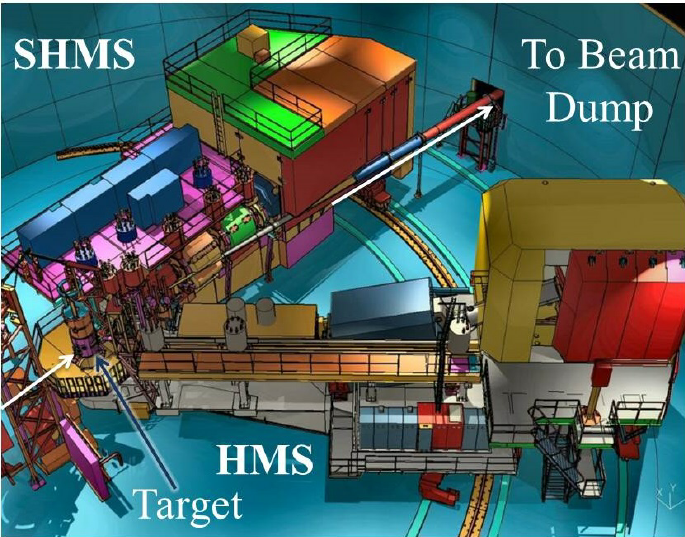
\includegraphics[width=0.5\textwidth]{hallc_spectrometer.png}}}%
    \caption{JLab experiment hall overview}%
    label{hallc_spectrometer}
  \end{figure}    
In this experiment we measured CSV effect at several $Q^2$ (4,4.7,5.5$GeV^2$) setting, for each $Q^2$ setting, we have x for $0.35-0.5$, $0.45-0.6$ and $0.5-0.65$ respectively, and z from 0.4 to 0.7.
\section{Conclusion}
This experiment can place constraints on charge symmetry violation in quark distribution functions by measuring pion ratios. The existance of charge symmetry violation effect can add another term on parton distribution function.  Also, this experiment can enrich the semi-inclusive data set for HallC  as part of the overall JLab semi-inclusive program. 

\medskip

\bibliographystyle{unsrt}
\bibliography{M335.bib}

\end{document}
